% !TEX root = ../thesis-example-en.tex
\chapter{The nitrogen vacancy center in diamond}\label{sec:nvc_diamond}

\section{Diamond as a host}
Diamonds have maintained their relevance throughout history, first and today as a gemstone, then for industrial and scientific tooling, and now in quantum technologies\cite{markhamDiamondQuantumRevolution2020}. The detection and control of single negatively charged nitrogen-vacancy (NV$^-$)\cite{gruberScanningConfocalOptical1997} color centers in diamond in 1997 marks the entry of diamond into quantum technologies\cite{dohertyNitrogenvacancyColourCentre2013}. The properties of diamond as a host directly lend to the success of the NV center in quantum technologies. The properties are introduced here.

Diamond is a crystal of carbon atoms with tetrahedral $sp^3$ hybrid orbital, present in a rigid face-centered cubic (fcc) lattice. It presents a high thermal conductivity of \qty{22}{\watt\centi\meter^{-1}\kelvin^{-1}}. Intrinsic diamond is a wide band gap semiconductor (\qty{5.48}{\electronvolt}), making it transparent in the visible spectrum. High concentration of defects lead to colored diamond, often found in nature. Commonly occurring colors are purple (NV), yellow (N), green (vacancies), and blue (B)\cite{DiamondsNatureGuide,mildrenIntrinsicOpticalProperties2013}.

Diamond, due to its highly stable chemical structure is very stable and inert, bio-compatible, and therefore suitable for biological applications\cite{wuDiamondQuantumDevices2016}.

The Debye temperature of diamonds is \qty{1860}{\kelvin}, resulting in a low phonon density of state at room temperature, providing a low spin-phonon decoherence environment for spin defects. The nuclear spin and paramagnetic spin abundance determines the spin-noise  environment. The lattice contains the spin free \ce{^{12}C} isotope (98.9\% natural abundance) and \ce{^{13}C} isotope with nuclear spin $I=1/2$. The \ce{^{13}C} isotope concentration can be depleted to 0.3\% and the paramagnetic impurity concentration can be $<\qty{e13}{\centi\meter^{-3}}$ for isotopically engineered diamonds\cite{balasubramanianUltralongSpinCoherence2009}.

Diamonds for quantum technologies, presenting low defect concentration (the most common being nitrogen), can be broadly classified into two types based on the amount of this concentration. Type I diamonds present nitrogen impurities in concentrations $>\qty{5}{ppm}$. Further, type Ia diamonds present nitrogen aggregates, and type Ib presents single nitrogen atom defects (P1 centers). Type II diamonds are the purest, containing $<\qty{5}{ppm}$ of nitrogen and mostly only carbon for type IIa and boron impurities in type IIb\cite{sunDiamondMEMSClassical2023}.

These diamonds can be created by mainly two methods: high-pressure high-temperature (HPHT) growth\cite{sauerSyntheticDiamondBasic1999} and chemical vapour deposition (CVD)\cite{schwanderReviewDiamondSynthesis2011} growth. Depending on the growth parameters precise control of the properties of the diamond is possible\cite{osterkampEngineeringPreferentiallyalignedNitrogenvacancy2019}. These works lead to the availability of an excellent host material for spin defects in diamond.

A few challenges still remain, such as the high cost of large single crystalline diamonds, and its infancy in fabrication processes\cite{challierAdvancedFabricationSingleCrystal2018}, reliable and low proximal damage creation of defects\cite{santonocitoNVCentresVacancies2024}, and compatibility with other semiconductor technologies\cite{sunDiamondMEMSClassical2023}, all of which are is active areas of research.

\section{Nitrogen vacancy center}

The NV center is a substitutional nitrogen atom and an adjacent vacancy site in the diamond carbon lattice\cite{dohertyNitrogenvacancyColourCentre2013}. Photo-stability\cite{gruberScanningConfocalOptical1997}, single photon generation\cite{kurtsieferStableSolidStateSource2000}, and optically detected magnetic resonance allowing for spin state control of the center's electron and nearby nuclear spins\cite{jelezkoObservationCoherentOscillation2004,jelezkoObservationCoherentOscillations2004}, set the stage for the center's development as a solid state qubit and sensor. 

\begin{wrapfigure}{}{0.5\textwidth}
    \begin{center}
        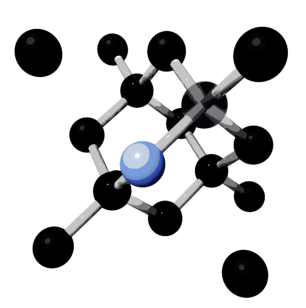
\includegraphics[width=0.5\textwidth]{../figures/nv_illust.pdf}
    \end{center}
        \caption[Structure of NV center]{Illustration of the structure of an NV center. The substitutional nitrogen atom (blue) is present adjacent to a vacancy (translucent). }
        \label{fig:nv_illust}
\end{wrapfigure}

% \begin{figure}
%     \centering 
%         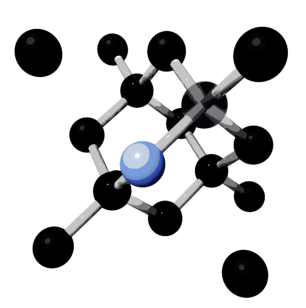
\includegraphics[width=0.5\textwidth]{../figures/nv_illust.pdf}

%         \caption[Structure of NV center]{Illustration of the structure of an NV center. The substitutional nitrogen atom (blue) is present adjacent to a vacancy (translucent). }
%         \label{fig:nv_illust}
% \end{figure}

The significance of the NV center is seen with some of the milestone achievements made possible by the center such as room temperature quantum registers\cite{neumannMultipartiteEntanglementSingle2008,duttQuantumRegisterBased2007}, spin-photon entanglement\cite{toganQuantumEntanglementOptical2010}, nanoscale magnetometry\cite{degenScanningMagneticField2008a,taylorHighsensitivityDiamondMagnetometer2008,maertzVectorMagneticField2010,steinertHighSensitivityMagnetic2010a}, bio-sensing\cite{schirhaglNitrogenVacancyCentersDiamond2014}, electrometry\cite{doldeElectricfieldSensingUsing2011a}, thermometry\cite{kucskoNanometrescaleThermometryLiving2013}, and relaxometry\cite{mzykRelaxometryNitrogenVacancy2022}. These findings continue to enable the use of the center as an excellent solid-state spin qubit and nanoscale-multi sensor\cite{degenQuantumSensing2017}.

The NV center exhibits $C_{3v}$ symmetry, meaning a 3-fold rotational symmetry along the NV axis and mirror symmetry. This allows for four possible NV orientations. In most diamonds, these structures appear with equal probability, although this probability can be engineered\cite{osterkampEngineeringPreferentiallyalignedNitrogenvacancy2019}. An illustration of the structure is shown in \cref{fig:nv_illust}.

The NV center exhibits two charge states, the negative charge state (NV$^{-1}$) with an electron spin of $S=1$ and a neutral charge state (NV$^0$) with an electron spin of $S=1/2$. The ZPL (zero phono line) represents the sharp, pure electronic transition between energy states in a solid-state defect, occurring without the emission or absorption of phonons. The NV$^{-1}$ ZPL is characteristic at \qty{637}{\nano\meter} and the NV$^0$ ZPL is at \qty{575}{\nano\meter}. They exhibit broad ($\sim \qty{100}{\nano\meter}$) phonon sidebands\cite{dohertyNitrogenvacancyColourCentre2013}. An example of the fluorescence spectrum is shown in \cref{fig:nv_zpl}.

\begin{figure}[h]
    \centering 
    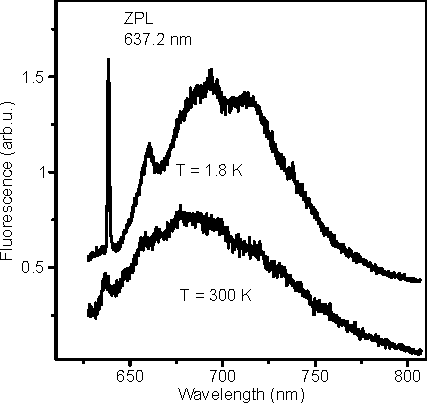
\includegraphics[width=0.75\textwidth]{../figures/nv_zpl.pdf}
    \caption[Fluorescence emission spectra of single NV centres]{Fluorescence emission spectra of single NV centres at room temperature and cryogenic temperatures. Excitation wavelength is \qty{514}{\nano\meter}. Reused with permission from John Wiley and Sons\cite{jelezkoSingleDefectCentres2006}.}
    \label{fig:nv_zpl}
\end{figure}

The NV center has 6 active electrons and the electronic states are a $^3$A$_2$ (spin triplet, non-degenerate) ground state (GS), $^3$E (spin triplet, doubly degenerate) excited state (ES) and two metastable shelving state, $^1$A and $^1$E (spin singlets)\cite{dohertyTheoryGroundstateSpin2012}, as shown in \cref{fig:jablosnki}. The transition between these states are shown in \cref{fig:jablosnki}. The ground state zero field splitting (ZFS) is $D_{{}^{3}\hspace{-0.8pt}\mathrm{A}_{2}} = \qty{2.87}{\giga\hertz}$ and the excited state splitting is $D_{{}^{3}\hspace{0pt}\mathrm{E}} = \qty{1.43}{\giga\hertz}$, lifting the degeneracy\cite{neumannExcitedstateSpectroscopySingle2009}. 

\begin{wrapfigure}{}{0.5\textwidth}
    \begin{center}
        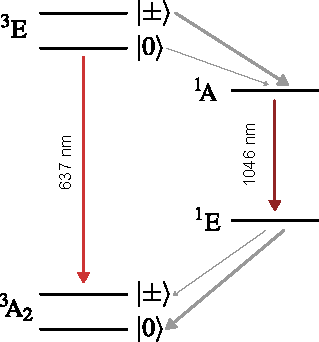
\includegraphics[width=0.5\textwidth]{../figures/jablonski.pdf}
    \end{center}
        \caption[Electronic structure of NV center]{Jablonski diagram of the electronic structure of the NV center. }
        \label{fig:jablosnki}
\end{wrapfigure}

The eigenstates of the spin triplet are given by the eigenstates of the $S_z$ operator, $m_s = 0, \pm1$  or $\ket{0},\ket{\pm}$. The inter-system crossing (ISC) decay path between ${}^{3}\hspace{0pt}\mathrm{E}$ and ${}^{1}\hspace{-0.8pt}\mathrm{A}$ and the difference in decay rates allow for spin state dependant fluorescence. The excited state lifetime for  $\ket{0}$ is $\tau_{\ket{0}}=\qty{23}{\nano\second}$ and for $\ket{\pm}$ is $\tau_{\ket{\pm}}=\qty{12.7}{\nano\second}$\cite{neumannExcitedstateSpectroscopySingle2009}, meaning a faster non-radiative decay into the shelving state ${}^{1}\hspace{-0.8pt}\mathrm{A}$ for $\ket{\pm}$. The shelving states decay with a lifetime of \qty{300}{\nano\second}\cite{rogersInfraredEmissionNV2008} to ${}^{3}\hspace{-0.8pt}\mathrm{A}_{2}$ GS via ISC. This non-radiative ISC to the GS is not spin conserving, and due to the higher ISC rate for the $\ket{\pm}$ state, the NV center is polarized into the $\ket{0}$ state under continuous optical excitation\cite{dohertyTheoryGroundstateSpin2012}. The ground state triplet is primarily exploited in this work as the sensing qubit. The grounds state spin Hamiltonian is given by
\begin{equation}
    H_{\mathrm{NV}} = D S_{z}^{2} + \gamma_{e} \mathbf{B} \cdot \mathbf{S},
\end{equation}

where $D = \qty{2.87}{\giga\hertz}$ is the GS ZFS, $\gamma_{e} = \qty{28.8}{\giga\hertz/\tesla}$ the electron gyromagnetic ratio ($2\pi$ omitted), $\mathbf{B}$ the magnetic field vector and $\mathbf{S}$ the electron spin operators. The intrinsic nitrogen in the NV center also provides a long-lived nuclear spin memory\cite{neumannMultipartiteEntanglementSingle2008}. It has two stable isotopes, \ce{^{14}N} (99.63\% natural abundance) and \ce{^{15}N} (0.37\% natural abundance). The Hamiltonian for interaction with \ce{^{14}N} is given by
\begin{equation}
    H_{\mathrm{hf\ ^{14}N}+^{14}N_{Zeeman}} = a_{\parallel} S_{z} I_{z} + a_{\perp} (S_{x} I_{x} + S_{y} I_{y}) + P I_{z}^{2} - \gamma_{\mathrm{^{14}N}} \mathbf{B} \cdot \mathbf{I},
\end{equation}

with the hyperfine terms being $a_{\parallel} = \qty{-2.14(7)}{\mega\hertz}$ and $a_{\perp} = \qty{-2.70(7)}{\mega\hertz}$, the quadrupole splitting $P = \qty{-5.01(6)}{\mega\hertz}$, $\gamma_{\mathrm{^{14}N}} = \qty{3.077}{\mega\hertz/\tesla}$ as the nitrogen gyromagnetic ratio, and $\mathbf{I}$ as the nuclear spin operator\cite{feltonHyperfineInteractionGround2009}.

For ultrapure CVD grown sample of type IIa diamond with $<\qty{5}{ppb}$ \ce{N}, the ground state spin coherence can extend from a few \qty{100}{\micro\second} to a few \unit{\milli\second} using dynamic decoupling\cite{childressCoherentDynamicsCoupled2006}, isotope engineering\cite{balasubramanianUltralongSpinCoherence2009}, or by n-type doping\cite{herbschlebUltralongCoherenceTimes2019}.

These mechanisms of spin state dependant fluorescence and optical spin polarization, along with coherent spin state control, establish the NV center as an excellent optically addressable qubit. A simple gated illumination and readout experiment shows these properties. \cref{fig:nv_odmr} shows such a measurement. The first $\sim\qty{300}{\nano\second}$ shows a significant differenct

\begin{wrapfigure}{}{0.5\textwidth}
    \begin{center}
        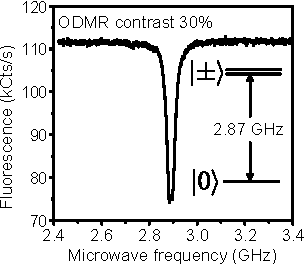
\includegraphics[width=0.5\textwidth]{../figures/odmr_line.pdf}
    \end{center}
        \caption[]{Reused with permission from John Wiley and Sons\cite{jelezkoSingleDefectCentres2006}.}
        \label{fig:nv_odmr}
\end{wrapfigure}

\begin{figure}[h]
    \centering 
    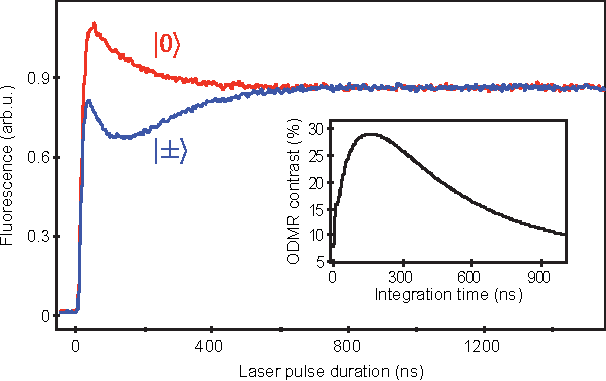
\includegraphics[width=0.95\textwidth]{../figures/odmrA.pdf}
    \caption[]{Reused with permission from American Physical Society\cite{dreauAvoidingPowerBroadening2011}.}
    \label{fig:pulsed_readout}
\end{figure}

\begin{wrapfigure}{}{0.5\textwidth}
    \begin{center}
        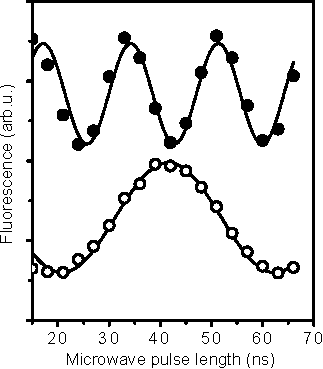
\includegraphics[width=0.5\textwidth]{../figures/rabi_osc.pdf}
    \end{center}
        \caption[]{Reused with permission from John Wiley and Sons\cite{jelezkoSingleDefectCentres2006}.}
        \label{fig:rabi_osc}
\end{wrapfigure}